\section{A Better Use of Audio-Visual Cues: Dense Video Captioning with Bi-modal Transformer}

\subsection{Overview}

\par Iashin and Rahtu, in their 2020 paper titled \textit{A Better Use of Audio-Visual Cues} \cite{iashin2020better},
approached the task of Dense Video captioning by using two types of input features: video as well as
audio. They identified the lack of research into utilizing the audio track of videos to generate
dense captions, despite the natural co-occurence of the two. They introduce a nove \textit{Bimodal
Transformer} which has the similar encoder-decoder architecture as the traditional Transformer model, 
but generalizes it to two input modalities:  audio features (using VGGish \cite{vggish}) and visual 
features (using I3D \cite{carreira2018quo}). Their  framework also consists of a \textit{multiheaded bimodal 
proposal generator}, inspired by the \textit{YOLO} object detector \cite{yolo} which generates event 
proposals for caption generation.


\subsection{Datasets}
\begin{itemize}
\item ActivityNet Captions \cite{krishna2017densecaptioning}
\end{itemize}

\subsection{Performance}
\par Iashin \textit{et al} report state-of-the-art-performance for the dense video captioning 
task on the published validation subset of the ActivityNet Captions dataset in terms of BLEU@3-4 
metrics and near state-of-the-art performance in terms of the METEOR metric. Considering the 
task of proposal generation in isolation, they report state-of-the-art performance with the F1 
score of 60.27\%, on the same dataset.


\subsection{Methodology}

\par Iashin \textit{et al} use a Inflated 3D Network pre-trained on the \textit{Kinetics} dataset
\cite{kay2017kinetics} for extracting visual features from video
frames. For audio features, the VGGish network \cite{vggish} is used. These features are stacked in 
sequence for each video. The caption tokens are embedded with pre-trained \textit{GloVe} \cite{glove}.

\begin{figure}[h]
	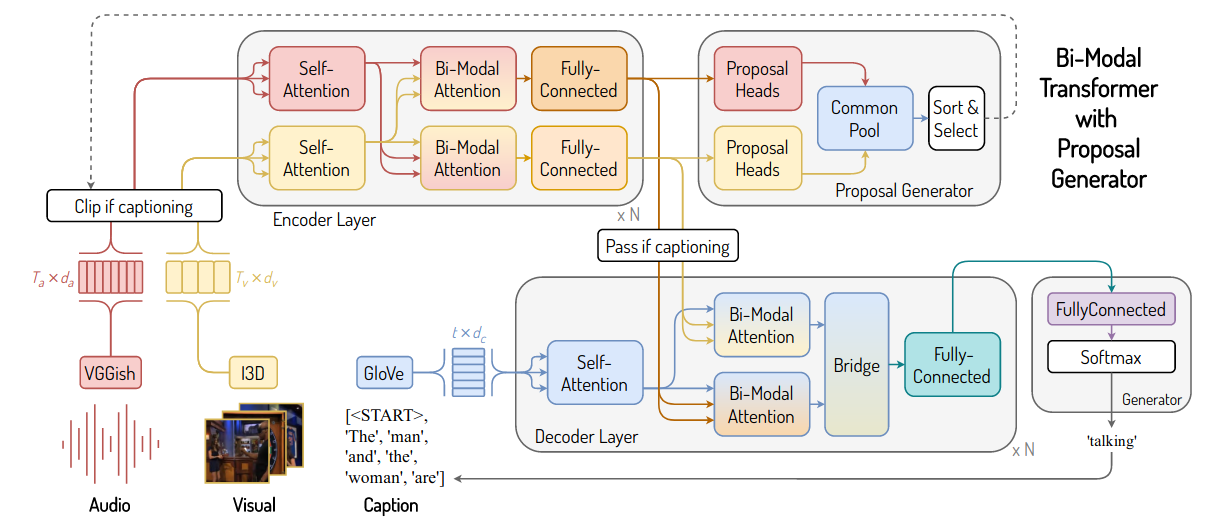
\includegraphics[width=\linewidth]{assets/img/bmt-architecture.png}
	\caption{Dense Video Captioning Framework introduced by Iashin \textit{et al} (Image courtesy \cite{iashin2020better})}
\end{figure}


\par The design proposed by Iashin \textit{et al} consists of two major functional components:
\begin{itemize}
\item Bi-modal Transformer
\item Multiheaded Proposal Generator
\end{itemize}

For inference, the features flow through the components as follows:
\begin{enumerate}
\item Both feature sequences, audio $A$ and visual $V$ are self-attended and then passed
through an $N$-layered encoder to produce bi-modal sequence representations using novel
bi-modal multi-headed attention blocks to fuse features from both sequences. These bimodal
attention blocks output two sequences of features, $A^v$ (visual attended audio features)
and $V^a$ (audio attended visual features).

\item $A^v$ and $V^a$ are then given to the Proposal Generator, which consists of two
distinct sets of \textit{proposal generator heads}, one set for each input modality.
Each proposal generator head makes proposal predictions at each time step independently,
forming a common pool of cross-modal predictions. Top $k$ predictions are selected (using a
confidence score) from this pool to be the output of the proposal generator: the proposals.

\item The generated proposals are used to clip the input feature sequences which are then
given to the Bimodal Encoder. The same self-attention followed by bimodal attention is
carried out on these clipped features.

\item The encoder's outputs are passed to the bi-modal attention blocks in every decoder
layer of the Bimodal Decoder, along with the representation of previously generated caption
words. The caption embeddings are self-attended, and then carries out bi-modal
encoder-decoder attention, producing $C_n^{A^v}$ (audio-visual attended previous captions)
and $C_n^{V^a}$ (visual-audio attended previous captions). After a bridge connection and
positional encoding (to add order information to the permutation invariant transformer
architecture), two fully connected layers with ReLU activation between them and a softmax
activation in the final layer are used to model the distribution of the next caption token 
over the vocabulary.

\end{enumerate}

\subsubsection{Proposal Generation Module}


\par The design of individual proposal generator heads in the Proposal Generator is inspired by 
the YOLO object detector \cite{yolo}. A set of anchors is determined apriori by running 
K-Means Clustering on the ground truth event lengths. Each centroid of the cluster is taken 
as an anchor in the anchor set $\psi$. The distance metric used here is the Euclidean 
distance, in contrast to IoU (Intersection over Union) used in YOLO. Each proposal generator 
head predicts three values: (1) center of the event $c$, (2) log coefficient $l$ and (3) 
objectness score $o$. Using these values, the temporal boundaries and confidence of the event 
predicted are calculated:

$$ center = p + \sigma(c) $$
$$ length = anchor\_length \cdot e^l $$
$$ confidence = \sigma(o) $$

\begin{figure}
	\centering
	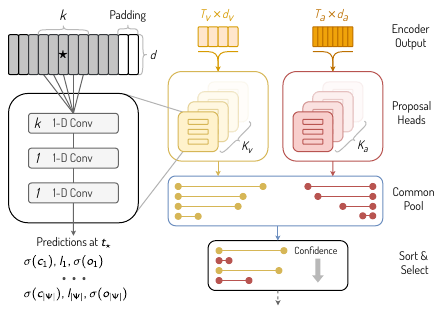
\includegraphics[width=0.8\linewidth]{assets/img/bmt-proposal-generator}
	\caption{Bi-modal Multiheaded Proposal Generator: Architecture (Image courtesy \cite{iashin2020better}}
\end{figure}

\par
Each proposal generator head consists of three 1D convolutional layers, through which the 
sequence length is preserved using padding and unit stride. The first convolutional layer 
has kernel size from a predetermined set of kernel sizes (calculated for each modality using 
K-Means clustering on event ground truth event lengths; the idea is to match receptive field 
sizes with event sizes). The other two layers have unit kernel size.\par

The loss for center $c$ and log coefficient $l$, collectively called \textit{Localization 
error} is the Mean Squared Error (MSE), while the confidence loss is a weighted sum of 
Binary Cross Entropy (BCE) of objectness and no-objectness loss. \par


\subsubsection{Captioning Module}
\par
The captioning module is essentially the Bimodal Transformer, consisting of a bimodal 
encoder and a bimodal decoder. The input to the bimodal encoder during captioning is feature 
sequences $A$ and $V$, which temporally correspond to a proposal. These two sequences go 
through $N$ encoder layers, each of which consist of (1) multiheaded self-attention of the 
two input sequences, (2) multiheaded bi-modal attention of the two sequences, giving $A^v$ 
and $V^a$ and then (3) two position-wise fully-connected layers with residual connections. 
These sublayers have separate trainable weights for both modalities.\par

The bimodal decoder is given the previous sequence of caption tokens as input, along with 
the output of the encoder $A^v_N$ and $V^a_N$. Each decoder layer consists of the following 
sublayers: (1) self-attention of caption tokens, (2) bimodal attention of captions with 
$A^v$ and $V^a$, (3) a bridge connection to concatenate and combine $C_n^{A^v}$ 
(audio-visual attended previous captions) and $C_n^{V^a}$ (visual-audio attended previous 
captions) and (4) two position-wise fully connected layers which act as the classification 
layers for the next caption token.\par


\subsubsection{Training Procedure}
\par
First, the captioning module is trained using ground truth proposals and their given 
captions using KL-divergence loss and label smoothing. The bimodal encoder weights are then 
frozen and then the proposal generator is trained using the trained bimodal encoder. Each 
proposal head uses Mean Squared Error for localization and binary cross-entropy for proposal 
loss.\par


\subsection{Conclusion}
\par The work by Iashin \textit{et al} provides a compelling case for exploring the use of 
multiple modalities for the task of Dense Video Captioning. Their ablation study shows that 
performance with using only visual features is more than using only audio features, 
indicating visual modality has a stronger signal for video understanding than audio 
modality; however, performance using both modalities gives consistently better results than 
single modalities in all settings.
